%! suppress = EscapeUnderscore
%! suppress = MissingLabel

Как-то Joe Fasel в разговоре с Philip Wadler высказал идею того, что перегрузка функций (overloading) должна находить своё отражение в типах.
Wadler понял его неправильно~\cite{hudak2007history}.
Но то, что он понял, --- оказалось классами типов~\cite{wadler1989make}.

Christopher Strachey ввёл классификацию полиморфизма на две категории.
Параметрический --- один и тот же код работает с данными различных типов.
\vocab{Специальный (ad-hoc) полиморфизм} --- код выбирается в зависимости от типа.
Например, один и тот же символ умножения по-разному действует на целые числа и на числа с плавающей точкой.

Перегрузка в языках обозначает возможность назвать несколько функций одинаково, у которых должны быть различные наборы входных параметров.
В месте вызова компилятор статически определяет по типам аргументов, какую из них действительно следует вызвать.
\begin{minted}{cpp}
    string toString(x: int) { ... }
    string toString(fmt: String, d: double) { ... }
\end{minted}

Классы типов обязуют сначала задекларировать именованную сущность (собственно, класс типов), включающую в себя пачку деклараций функций, которые могут быть перегружены для различных типов.
\begin{minted}{haskell}
    class Show a where
      show :: a -> String

    instance Show Int where
      show :: Int -> String
      show = ...
\end{minted}

Необходимо заметить, что декларация класса типов содержит формальный типовой параметр, по вхождениям которого в тип функции, собственно, выбирается перегрузка.
Таких параметров может быть много, они могут иметь стрелочные кайнды.
Например, в случае класса типов \mintinline{haskell}|Applicative|, выбор реализации операции \mintinline{haskell}|pure| будет происходить по типовому конструктору результата, то есть даже не по полноценному типу.
Такая гибкость и близко не достигается при классической перегрузке.
\begin{minted}{haskell}
    class Functor f => Applicative (f :: Type -> Type) where
      pure :: a -> f a
      ...

    instance Applicative Maybe where
      pure :: a -> Maybe a
      ...
\end{minted}

Также, в отличие от перегрузки, классы типов совместимы с параметрическим полиморфизмом.
Так, в типе полиморфной функции нельзя указать, что для типа должна присутствовать определённая перегрузка.
Классы типов же позволяют ограничить набор возможных типовых аргументов теми, для которых реализован инстанс нужного класса типов:
\begin{minted}{haskell}
    showPrefixed :: Show a => a -> String -> String
\end{minted}

Если сравнивать классы типов с переопределением (overriding) в ООП языках, то разрешение вызова виртуальной функции происходит с использованием таблицы, хранящейся объекте первого параметра (получателя вызова, receiver).
Классы типов же опираются исключительно на тип, поэтому, например, возможно определение констант в классах типов:
\begin{minted}{haskell}
    class Enum a => Bounded a where
      minBound :: a
      maxBound :: a
\end{minted}

В то же время, классы типов не являются типами, а, скорее, предикатами на типах.
Тип удовлетворяет такому предикату, или свойству, если для него есть соответствующий инстанс.
Поэтому, в частности, привычный способ в ООП создать гетерогенную коллекцию элементов, имеющих общий интерфейс, напрямую не сработает с классами типов.
Например, такой тип не будет корректным: \mintinline{haskell}|[Show]|.
Мы вернёмся к этой проблеме в~\ref{subsubsec:existentials}.

\subsection{Устройство классов типов}

Несмотря на поразительное могущество, идея реализации классов типов крайне проста.
Она была уже во всей полноте представлена в первой работе~\cite{wadler1989make}.
В дальнейших работах уточнялся механизм вывода типов в виде сведения к классической системе типов в стиле Hindley-Milner~\cite{hall1996type}.
Остальные работы, в основном, предлагают огромное разнообразие различных приложений.

\subsubsection{Словари}

Рассмотрим идею реализации классов типов на примере полиморфной сортировки.
Сортировка для списка элементов конкретного типа пишется тривиально:
\begin{minted}{haskell}
    sort :: [Int] -> [Int]
    sort = \case [] -> []; x:xs -> insert x (sort xs)
      where
        insert x xs = let (l, r) = List.partition (?\framebox{<}? x) xs in l ++ x : r)
\end{minted}

В реализации единственная информация о типе, которой мы пользуемся --- порядок на его обитателях.
Таким образом, при переходе к полиморфной сортировке, нам нужно принять словарь с предикатами, задающими нужный порядок для данного типа\footnote{Приятный синтаксис распаковки рекордов доступен с расширением \href{https://ghc.gitlab.haskell.org/ghc/doc/users_guide/exts/record_wildcards.html}{RecordWildCards}.}.
\begin{minted}{haskell}
    data OrdDict a = OrdDict { less :: a -> a -> Bool }

    sort :: OrdDict a -> [a] -> [a]
    sort d@OrdDict {..} = \case [] -> []; x:xs -> insert x (sort d xs)
      where
        insert x xs = let (l, r) = List.partition (?\framebox{`less`}? x) xs in l ++ x : r
\end{minted}

Теперь, чтобы воспользоваться сортировкой на списке чисел, нужно сконструировать нужный рекорд и вызвать с ним функцию на списке конкретных типов:
\begin{minted}{haskell}
    intOrd :: OrdDict Int
    intOrd = OrdDict { less = (<) }

    ghci> sort intOrd [3, 2, 1]
\end{minted}

Возможна ситуация, когда инстанс для одного типа зависит от инстанса для другого
Например, сравнение списков можно получить автоматически, зная порядок на элементах.
В случае словарей мы это моделируем функцией между словарями:
\begin{minted}{haskell}
    listDict :: OrdDict a -> OrdDict [a]
    listDict d = OrdDict { less = ... ?\framebox{less d}? ... }
\end{minted}

Теперь мы можем сортировать список списков, конструируя нужный словарь:
\begin{minted}{haskell}
    ghci> sort (listDict intDict) [[3, 2], [2, 1], [0]]
\end{minted}

Сравнение явной передачи словарей и классов типов можно увидеть в следующей таблице:

\begin{tabular}{p{8cm}p{8cm}}
    \begin{enumerate}
        \item Определение словаря функций
        \begin{minted}{haskell}
            data MyOrd a = MyOrd
              { less :: a -> a -> Bool }
        \end{minted}
        \item Экземпляр словаря для конкретного типа
        \begin{itemize}
            \item Именованное значение
        \end{itemize}
        \begin{minted}{haskell}
            intMyOrd :: MyOrd Int
            intMyOrd = MyOrd { less = (<) }
        \end{minted}
        \item Явный параметр функции
        \begin{minted}{haskell}
            sort :: MyOrd a -> [a] -> [a]
        \end{minted}
        \item Передаётся пользователем
        \begin{minted}{haskell}
            test = sort ?\framebox{intMyOrd}? [3, 2, 1]
        \end{minted}
    \end{enumerate}
    &
    \begin{enumerate}
        \item Определение класса типов
        \begin{minted}{haskell}
             class MyOrd a where
               less :: a -> a -> Bool
        \end{minted}
        \item Объявление типа представителем класса типов
        \begin{itemize}
            \item Не имеет имени
        \end{itemize}
        \begin{minted}{haskell}
            instance MyOrd Int where
              less = (<)
        \end{minted}
        \item Неявный параметр функции
        \begin{minted}{haskell}
            sort :: MyOrd a => [a] -> [a]
        \end{minted}
        \item Передаётся компилятором
        \begin{minted}{haskell}
            test = sort [3, 2, 1]
        \end{minted}
    \end{enumerate}
\end{tabular}

Таким образом, словарь --- это свидетель (witness) того, что тип удовлетворяет ограничению.
Подобно тому, как коерции свидетельствуют несинтаксические эквивалентности на типах~\ref{subsubsec:gadts}.

\begin{task}
    Какой словарь будет соответствовать higher-kinded классу типов \mintinline{haskell}|Functor|?
\end{task}

\subsubsection{Неявные аргументы}

Можно думать так, что слева от \mintinline{haskell}|=>| передаются неявные аргументы функций, выводимые компилятором из контекста.
То есть, например, не стоит удивляться вхождениям \mintinline{haskell}|=>| в отрицательной позиции, это просто функция с неявным аргументом.
Так, следующий код не скомпилируется, потому что в месте использования переменной \texttt{y} нет значения типа \mintinline{haskell}|Show b|:
\begin{minted}{haskell}
    f :: (Show b => b) -> b
    f x = ?\framebox{x}?
\end{minted}
Можно это значение принять в функции \texttt{f}, тогда оно автоматически пропагируется в \texttt{y}:
\begin{minted}{haskell}
    f :: Show b => (Show b => b) -> b
    f x = ?\framebox{x}?
\end{minted}

Расширение \href{https://ghc.gitlab.haskell.org/ghc/doc/users_guide/exts/implicit_parameters.html}{ImplicitParams} даёт возможность делать некоторые аргументы функции неявными.
Фактически, это реализация динамического связывания в статическом языке~\cite{lewis2000implicit}.
Неявные аргументы берутся из скоупа по имени и подставляются автоматически:
%! suppress = EscapeHashOutsideCommand
\begin{minted}[escapeinside=##]{haskell}
    sortBy :: (a -> a -> Bool) -> [a] -> [a]

    sort :: (?cmp :: a -> a -> Bool) => [a] -> [a]
    sort = sortBy ?cmp
\end{minted}

Haskell также предоставляет возможность сохранять словари в структуры данных:
\begin{minted}{haskell}
    data ShowDict a where
      ShowDict :: Show a => ShowDict a

    f :: ShowDict b -> (Show b => b) -> b
    f d x = case d of ShowDict -> ?\framebox{x}? -- в скоупе доступен инстанс Show b
\end{minted}

\begin{task}
    Возможна ли именно такая семантика в энергичном языке?
    Почему?
\end{task}

\subsubsection{Вывод инстансов}

Чтобы вызвать ограниченно-полиморфную функцию, GHC производит вывод инстансов или, иначе говоря, автоматически конструирует свидетелей.
Вывод инстансов тесно интегрирован с общей системой вывода типов Haskell~\cite{spj-type-inference}.

В действительности вывод инстансов это не что иное, как \point{задача населения типа}.
Действительно, после трансляции в Core (промежуточное представление в GHC), классы типов представляют собой словари функций.
У нас в контексте имеются конкретные словари и функции, позволяющие из одних словарей получать другие.
Требуется найти терм, конструирующий словарь нужного типа.

Например, внутри функции \mintinline{haskell}|f :: Show a => ..| происходит вызов ограниченно- полиморфной функции
\mintinline{haskell}|g :: Show [a] -> ..|.
У нас имеется словарь \mintinline{haskell}|ShowDict a|, а так же функция \mintinline{haskell}|ShowDict a -> ShowDict [a]|, пришедшая из импортов\footnote{Инстансы можно импортировать пустым импортом: \mintinline{haskell}|import Module ()|.}.
Необходимо сконструировать терм типа \mintinline{haskell}|ShowDict [a]|.
Очевидно, это будет просто аппликации одного к другому.

Вывод инстансов происходит рекурсивно.
Чтобы вывести \mintinline{haskell}|ShowDict [a]|, выводится сначала посылка \mintinline{haskell}|ShowDict a|.
То есть получается рекурсия по структуре типа.
Иначе говоря, вывод инстансов можно эксплуатировать как вычислительный примитив уровня типов.
Так, например, мы можем опускать информацию из типов в термы (аналогично в \href{https://hackage.haskell.org/package/base-4.20.0.1/docs/GHC-TypeLits.html}{GHC.TypeLits}).
\begin{minted}{haskell}
    type data Nat = Zero | Suc Nat

    class KnownNat (n :: Nat) where
      natVal :: Int

    instance KnownNat Zero where
      natVal = 0

    instance KnownNat n => KnownNat (Suc n) where
      natVal = 1 + natVal @n

    ghci> natVal @(Suc (Suc Zero))
    -- выведется natVal {knownSuc (knownSuc knownZero)}
\end{minted}

В общем случае процесс населения типа, как можно предположить по вычислительной аналогии, неразрешим.
Поэтому GHC накладывает большое количество ограничений на вид инстансов, которые гарантируют тотальность вывода.
Подробно эти ограничения описаны в~\cite{sulzmann2007understanding}.
Также GHC предоставляет различные расширения, ослабляющие эти ограничения и перекладывающие часть ответственности на плечи программиста\footnote{\url{https://downloads.haskell.org/ghc/latest/docs/users_guide/exts/instances.html}}.
Например, c UndecidableInstances можно легко написать разворот списка типов на этапе компиляции, как и любую другую функцию:
\begin{minted}{haskell}
    class Reverse (acc :: [Type]) (tys :: [Type]) where
      showReverse :: String

    instance ShowT acc => Reverse acc '[] where
      showReverse = showTypes @acc

    instance Reverse (ty : acc) tys => Reverse acc (ty : tys) where
      showReverse = showReverse @(ty : acc) @tys

    ghci> showReverse @'[] @'[Char, Int, Double]
\end{minted}

Между классами типов и выводом типов существует интересная синергия (рис.~\ref{fig:class-sinergy})\footnote{\href{https://youtu.be/5QQdI3P7MdY?si=VAgqyD7iycALTrz_}{(youtube) Hackett: a metaprogrammable Haskell}.}.
Исходя из термов, выводятся типы.
Исходя из типов, выводятся инстансы классов типов.
То есть мы пишем какой-то интересный интеллектуальный код, а параллельно с нами компилятор выписывает неинтересный код.

\begin{figure}
    \centering
    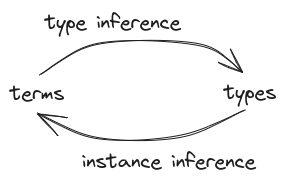
\includegraphics[width=0.4\textwidth]{figs/class-sinergy}
    \caption{Классы типов + вывод инстансов = кодогенерация.}
    \label{fig:class-sinergy}
\end{figure}

Вывод инстансов опирается только на вид ``головы'' декларации --- справа от \mintinline{haskell}|=>|, а ограничения слева применяются постфактум.
Это можно использовать, чтобы писать более общие инстансы.
Так, например, работает \vocab{constraint trick}\footnote{\url{https://chrisdone.com/posts/haskell-constraint-trick/}}, позволяющий резолвить ad-hoc полиморфные функции в параметрически-полиморфном контексте.

Этим же пользуется механизм программируемых ошибок компиляции из \href{https://hackage.haskell.org/package/base-4.20.0.1/docs/GHC-TypeLits.html}{GHC.TypeLits}.
Если инстанс сработал и компилятор начал обрабатывать ограничения слева, значит, что-то пошло не так~\cite[глава 12]{maguire-types}.

\begin{minted}{haskell}
    instance (TypeError
      ( Text "Attempting to show a function of type "
        :<>: Text "'" :<>: ShowType (a -> b) :<>: Text "'"
        :$$: Text "Did you forget to apply an argument?"
      )) => Show (a -> b) where
      show = undefined -- реализация не важна, до исполнения дело не дойдёт
\end{minted}

\subsubsection{Построение типа по значению} \label{subsubsec:reify}

После того как мы научились опускать значения из типов, закономерно научиться обратному --- поднимать значения в типы.

Рассмотрим вспомогательную концепцию проксирования.
В стандартной библиотеке определён тип \mintinline{haskell}|Proxy| с одним фантомным параметром.
Исторически он нужен, чтобы обходить отсутствие расширений \href{https://downloads.haskell.org/ghc/latest/docs/users_guide/exts/type_applications.html#extension-TypeApplications}{TypeApplications} и \href{https://downloads.haskell.org/ghc/latest/docs/users_guide/exts/type_abstractions.html#extension-TypeAbstractions}{TypeAbstractions}.
А именно --- неинформативную константу \mintinline{haskell}|Proxy| можно проаннотировать нужным типом и передать в функцию, чтобы специализировать типовой параметр на нужный тип.
Или принять \mintinline{haskell}|Proxy| и воспользоваться \href{https://downloads.haskell.org/ghc/latest/docs/users_guide/exts/scoped_type_variables.html#pattern-type-signatures}{ScopedTypeVariables} для типовых сигнатур в паттернах.
\begin{minted}{haskell}
    data Proxy (a :: k) = Proxy

    id :: Proxy a -> a -> a
    ghci> :t id (Proxy :: Proxy Int)
    id (Proxy :: Proxy Int) :: Int -> Int

    id (Proxy :: Proxy ?\framebox{a}?) x = (x :: ?\framebox{a}?)
\end{minted}

Иногда прокси-тип оставляют полиморфным, чтобы пользователь сам мог его задать.
Вместо конкретного значения иногда передают специализированное значение $\bot$, а получатель, не зная тип, не сможет его форсировать (однако, любые вхождения $\bot$ в тип слишком настораживают).
\begin{minted}{haskell}
    id :: proxy a -> a -> a
    id (_ :: proxy a) x = (x :: a)

    ghci> :t id (undefined :: Proxy Int)
    id (undefined :: Proxy Int) :: Int -> Int
\end{minted}

Теперь напишем функцию поднятия значения в тип с помощью техники через полиморфную рекурсию, описанную в~\cite{kiselyov2004functional}.
Существует соответствующая библиотека\footnote{\url{https://hackage.haskell.org/package/reflection-2.1.6/docs/Data-Reflection.html}}.

В действительности мы, конечно, не можем честно получить синтаксически тип нужного размера, просто потому, что типы существуют строго до стадии исполнения.
Однако, как мы знаем, словари классов типов имеют воплощение в рантайме (случай полиморфной рекурсии~--- как раз пример, когда этого нельзя полностью избежать).
Поэтому воспользуемся continuation passing style, который будет подробно рассмотрен в главе~\ref{sec:continuations}: вместо того, чтобы вернуть результат, примем продолжение, умеющее работать с любым типом с \mintinline{haskell}|KnownNat|:
\begin{minted}{haskell}
    reify :: Int -> (forall n. KnownNat n => Proxy n -> a) -> a
    reify n k
      | n <= 0 = k (Proxy @Zero)
      | otherwise = reify (n - 1) \(Proxy :: Proxy n) -> k (Proxy @(Suc n))
\end{minted}

Продолжение, передаваемое в рекурсивный вызов, неявно принимает словарь для типа \texttt{n} и конструирует словарь для \mintinline{haskell}|Suc n|.

Наконец, можем написать следующую удивительную тождественную функцию, поднимающую сначала значение в тип, а потом опускающее тип обратно в термы:
\begin{minted}{haskell}
    wonderId :: Int -> Int
    wonderId n = reify n (\(Proxy :: Proxy n) -> natVal @n)
\end{minted}

\subsubsection{Имплиситы и когерентность}

Существуют подходы к реализации классов типов, когда они не являются отдельной возможностью языка, а получаются как следствие других, более общих, механизмов.

Так, в Scala существует механизм имплиситов (implicits)~\cite{kvrikava2019scala}.
Параметры функции могут быть помечены \mintinline{scala}|implicit|.
Теперь, если в контексте есть \mintinline{scala}|implicit| значения и \mintinline{scala}|implicit| функции, аргументы сгенерируются автоматически исходя из типа параметра.
Теперь мы можем смоделировать словарь функций, например, с помощью интерфейсов (которые в Scala называются \mintinline{scala}|trait|) и синглтонов, чтобы получить вполне себе классы типов~\cite{oliveira2010type}.
Функции с имплисит-параметрами не являются в полном смысле функциями первого класса в Scala.
\begin{minted}{scala}
    trait Show[T] {
        def show(x: T): String
    }

    def show[T](x: T)(implicit ev: Show[T]): String = ev.show(x)

    implicit object intShow extends Show[Int] {
        def show(x: Int): String = x.toString
    }

    def showAll[T](xs: List[T])(implicit ev: Show[T]): String =
        xs.map(show(_)).join(", ")
\end{minted}

В языках с зависимыми типами неявные параметры\footnote{\url{https://agda.readthedocs.io/en/v2.7.0.1/language/implicit-arguments.html}} особенно нужны, потому что, например, типы --- это такие же параметры функции, как и все остальные.
Поэтому вывод типов~--- это фактически вывод неявных аргументов функций.
Более того, зависимые функции, вместе с аргументами часто принимают доказательства каких-то свойств этих аргументов, которые тоже хочется по возможности выводить из контекста автоматически.
В свете аналогии между классами типов как предикатами на типах, а инстансами как доказательствами, свидетельствующими о выполнении предиката для типа, можно тот же механизм вывода доказательств переиспользовать для эмулирования классов типов\footnote{\url{https://agda.readthedocs.io/en/v2.7.0.1/language/instance-arguments.html}}~\cite{devriese2011bright}.
В обратную сторону можно механизмы зависимой типизации эмулировать классами типов~\cite{mcbride2002faking}.

Выражение классов типов через другие механизмы может выглядеть как абсолютно выигрышная стратегия на фоне реализации их как самостоятельной возможности языка.
Действительно, можно переиспользовать всё то могущество программирования, которое есть с рекордами, в то время как для классов типов и констреинтов то же самое приходится развивать отдельно\footnote{\url{https://downloads.haskell.org/ghc/latest/docs/users_guide/exts/instances.html}}.
Да и неявные аргументы, наверное, полезный механизм сам по себе.

Однако у подхода Haskell есть важное свойство при соблюдении всех ограничений, т.е. при отсутствии \vocab{orphan instances}\footnote{\url{https://stackoverflow.com/questions/3079537/orphaned-instances-in-haskell}}.
\vocab{Когерентность инстансов (coherence)} --- для одного типа все инстансы данного класса типов, полученные разными способами, неотличимы (рис.~\ref{fig:coherence}).
Соответственно, не имеет значения происхождение того или иного инстанса.
Иначе говоря, об этом можно не думать, это снимает существенное количество когнитивной нагрузки и упрощает рефакторинг\footnote{\href{https://youtu.be/hIZxTQP1ifo?si=aG2Lk2eb-5E5SOLb}{Edward Kmett - Type Classes vs. the World.}}.
В то время как остальные подходы требуют трепетного отношения к контексту вызова, потому что из него может прийти неожиданная реализация.

\begin{figure}
    \centering
    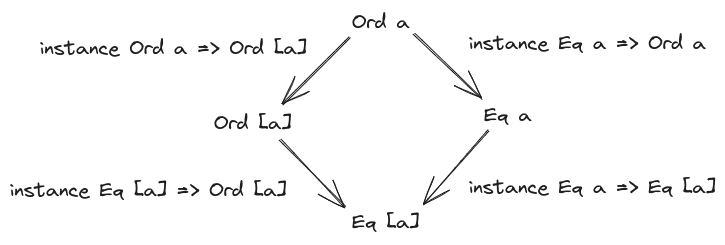
\includegraphics[width=0.8\linewidth]{figs/coherence}
    \caption{Когерентность инстансов --- диаграмма коммутирует.}
    \label{fig:coherence}
\end{figure}

\subsubsection{Правила (rules) и специализация}

GHC позволяет прямо в коде, с помощью специально прагмы, указывать оптимизирующие правила переписывания для компилятора\footnote{\url{https://downloads.haskell.org/ghc/latest/docs/users_guide/exts/rewrite_rules.html}}.
Например:
\begin{minted}{haskell}
    {-# RULES
      "map/map"    forall f g xs.  map f (map g xs) = map (f . g) xs
      "map/append" forall f xs ys. map f (xs ++ ys) = map f xs ++ map f ys
     #-}
\end{minted}

Первый закон представляет собой не что иное, как закон функторов.
В идеале, мы формулируем законы на этапе дизайна~\cite{maguire-algebra}, проверяем их выполнение с помощью property-based testing\footnote{\href{https://youtu.be/G0NUOst-53U?si=vdcKVUi9vSPBY0Jz}{(youtube) John Hughes - Keynote: How to specify it!}}, а потом используем их для оптимизаций.

Можно переписать полиморфную версию функции на специализированную, если типы подходят.
Для этого нужно реализовать специализированную версию (совпадение семантики --- полностью ответственность программиста) и задать соответствующее правило переписывания:
\begin{minted}{haskell}
    genericLookup :: Ord a => Table a b   -> a   -> b
    intLookup     ::          Table Int b -> Int -> b

    {-# RULES "genericLookup/Int" genericLookup = intLookup #-}
\end{minted}

Основной эффект такой оптимизации --- гарантированное превращение динамических вызовов функций классов типов в статические (потому что тип известен, следовательно, --- и соответствующий ему словарь).

\subsection{Семейства, ассоциированные семейства}

Идея ad-hoc полиморфизма в том, чтобы в зависимости от типа исполнялся различный код.
Семейства начинались как продолжение этой идеи в плоскость данных и типов.
Так, ассоциированные синонимы типов --- различные типы для различных индексов (типовых параметров)~\cite{chakravarty2005associated-syn}.
Ассоциированные \mintinline{haskell}|data| --- различные представления для различных индексов~\cite{chakravarty2005associated}.
В конце концов эти идеи были обобщены до открытых семейств~\cite{schrijvers2008type}, потом были введены открытые~\cite{eisenberg2014closed}.

Можно считать, что семейства\footnote{\url{https://ghc.gitlab.haskell.org/ghc/doc/users_guide/exts/type_families.html}}\footnote{\url{https://serokell.io/blog/type-families-haskell}} --- это типовые конструкторы, задающие множество типов.
Конкретный тип из множества можно выбрать, передав типовой параметр, называемый \vocab{индексом}.
Сравните с обычными полиморфными конструкторами типа, которые ведут себя одинаково вне зависимости от типовых параметров.

Большое количество примеров использований можно увидеть, например, в~\cite{kiselyov2010fun}.

\subsubsection{Data families}

Data families позволяют выбирать декларацию алгебраического типа в зависимости от типового индекса.
Например, для более эффективной реализации структур данных.
Это напоминает специализацию шаблонов в C++.

\begin{minted}{haskell}
    data family XList elem
    data instance XList () = IntList Int
    data instance XList Bool = ByteArray [Bool]
\end{minted}

Единственный способ работать с data family --- разместить реализацию в классе типов, чтобы она сопровождала значение с того момента, когда типовой индекс конкретный.

\begin{minted}{haskell}
    class XListOp elem where
      xelem :: elem -> XList elem -> Bool

    instance XListOp () where
      xelem () (IntList size) = size > 0

    instance XList Bool where
      xelem key (ByteArray bs) = key `elem` bs

    xelemAll :: XListOp elem => XList elem -> [elem] -> Bool
    xelemAll xs = all (`xelem` xs)
\end{minted}

\subsubsection{Synonym families}

Synonym families (семейства типов) фактически являются функциями на типах.
Они бывают открытыми, закрытыми и ассоциированными.
Открытые семейства открыты в том смысле, что инстансы можно писать отдельно от декларации, подобно классам типов.
Закрытые, наоборот, полностью описываются в одном месте, кейсы упорядочены сверху вниз, что несколько ослабляет ограничения на паттерны.

\begin{minted}{haskell}
    type family Plus (n :: Nat) (m :: Nat) :: Nat where
      Plus Zero m = m
      Plus (Suc n) m = Suc (Plus n m)
\end{minted}

Чтобы посмотреть, во что вычисляется нечто на уровне типов, можно воспользоваться следующей командой в ghci:
\begin{minted}{haskell}
    ghci> :k! Plus (Suc Zero) (Suc (Suc Zero))
    Plus (Suc Zero) (Suc (Suc Zero)) :: Nat
    = Suc (Suc (Suc Zero))
\end{minted}

Ассоциированные семейства работают аналогично, только объявляются в рамках некоторого класса типов, являясь некоторой функциональной альтернативой \href{https://ghc.gitlab.haskell.org/ghc/doc/users_guide/exts/functional_dependencies.html}{FunctionalDependencies} (которые выглядят скорее реляционно).
Иначе говоря, позволяют поставить в соответствие типу, для которого написан инстанс, другой тип.
Например, коллекции --- тип её элементов.

\begin{minted}{haskell}
    class Container a where
      type Elem a
      elements :: a -> [Elem a]

    instance Container [a] where
      type Elem [a] = a
      elements = id

    instance Container ByteString where
      type Elem ByteString = Word8
      elements = ByteString.unpack
\end{minted}

В современных языках часто встречаются ассоциированные семейства под видом ассоциированных типов.
Так, Swift сильно полагается на ассоциированные типы, вовсе не поддерживая дженерики в протоколах (интерфейсах)\footnote{\href{https://youtu.be/ctS8FzqcRug?si=y_ZYnuUOulA33d_X}{(youtube) 2017 LLVM Developers’ Meeting: ``Implementing Swift Generics''}}.
В то же время Scala пытается отслеживать, в присутствии экзистенциальных типов (интерфейсов), из какого именно значения пришёл тот или иной ассоциированный тип с помощью path-dependent types~\cite{amin2014foundations}.

\subsubsection{Инъективные семейства}

Семейства типов отличаются от типовых конструкторов примерно так же, как функции от конструкторов данных.
Конструкторы пассивны и не редуцируются (\mintinline{haskell}|Maybe Int|), в то время как функции вычисляются в какой-то результат (e.g. \mintinline{haskell}|F Int ?$\sim$? Bool|).
В частности, как и функции, семейства не обязательно инъективны.

Для типовых конструкторов, зная, что сконструированные ими типы эквивалентны, можно вывести, что типовые аргументы эквивалентны тоже.
Например:
\begin{minted}{haskell}
    Maybe a ?$\sim$? Maybe b ?$\Rightarrow$? a ?$\sim$? b
\end{minted}

Очевидно, что для классов типов это свойство по умолчанию не выполняется:
\begin{minted}{haskell}
    type family NonInjective a where
      NonInjective Int = Double
      NonInjective Char = Double
\end{minted}

Haskell предоставляет явный синтаксис для объявления инъективных семейств типов, напоминающий функциональные зависимости в классах типов (\href{https://ghc.gitlab.haskell.org/ghc/doc/users_guide/exts/type_families.html#extension-TypeFamilyDependencies}{TypeFamilyDependencies})~\cite{stolarek2015injective}.
Конечно, компилятор проверит, что реализация инъективна.
Синтаксис требует связать результат именем через равенство и указать, что результат определяет какие-то из типовых индексов семейства:
\begin{minted}{haskell}
    type family InjectiveB a b = r | r -> b
      ...
\end{minted}

\subsubsection{Семейства первого класса}

Помимо инъективности, классы типов также не обязательно обладают свойством \vocab{generavity}, критически важным для вывода типов, --- один и тот же результат не обязательно получен из того же самого семейства:
\begin{minted}{haskell}
    f a ?$\sim$? g a ?$\Rightarrow$? f ?$\sim$? g
\end{minted}

Вместе инъективность и generavity --- \vocab{matchability}.
Когда Haskell работает с типом стрелочного кайнда, он подразумевает, что этот тип matchable.
Соответственно, семейства не могут передаваться в качестве параметров, а все их вхождения должны быть полностью применёнными ко всем аргументам (fully saturated).

Одним из способов обойти это ограничение является дефункционализация семейств~\cite{defunctionalization-slides, eisenberg2014promoting}.
Как мы и обсуждали ранее~\ref{subsubsec:defunctionalization}, вместо функции первого класса заводится некоторый символ, обозначающий её, и функция интерпретации, умеющая сделать действие, соответствующее этому символу.
В данном случае функцией интерпретации будет открытое семейство \mintinline{haskell}|Apply|.

В Haskell ведутся работы\footnote{\href{https://ghc-proposals.readthedocs.io/en/latest/proposals/0242-unsaturated-type-families.html}{GHC proposal: Unsaturated Type Families}.} по устранению saturation ограничения~\cite{kiss2019higher}.
Для этого нужно различать matchable и unmatchable типовые функции.
Это предлагается делать дополнительным индексированием стрелочных кайндов: $\to \equiv
\to^M, \twoheadrightarrow \equiv \to^U$.
И, конечно, эти индексы могут быть полиморфными.

\begin{minted}{haskell}
    data Matchability = Matchable | Unmatchable

    hMap
      :: forall (m :: Matchability) (c :: Type -> Constraint)
       . forall (f :: Type ->?$^m$? Type) (as :: [Type])
       . All as c => (forall a. c a => a -> f a) -> HList as -> HList (Map f as)
\end{minted}

\subsection{Кайнд Constraint}

% todo boxed constraints

Давно появлялись предложения добавить в GHC поддержку синонимов для констреинтов, семейств констреинтов и т.д~\cite{orchard2010haskell}.
В итоге был предложен\footnote{\url{https://gitlab.haskell.org/ghc/ghc/-/wikis/kind-fact}} и реализован\footnote{\url{http://blog.omega-prime.co.uk/2011/09/10/constraint-kinds-for-ghc/}} некоторый механизм унификации типов и констреинтов.
Таким образом, всё, что работало для типов, стало работать и для констреинтов.

В GHC с \href{https://downloads.haskell.org/ghc/9.2-latest/docs/html/users_guide/exts/constraint_kind.html}{ConstraintKinds} был добавлен специальный кайнд \mintinline{haskell}|Constraint|:
\begin{itemize}
    \item Класс типов конструирует констреинт: \mintinline{haskell}|Monad :: (Type -> Type) -> Constraint|;
    \item Эквивалентность является констреинтом: \mintinline{haskell}|(a ?$\sim$? b) :: Constraint|;
    \item Пустой кортеж констреинтов является констреинтом: \mintinline{haskell}|() :: Constraint|;
    \item Кортеж констреинтов является констреинтом: \mintinline{haskell}|(Eq a, a ?$\sim$? b) :: Constraint|.
\end{itemize}

Теперь, например, мы можем реифицировать словарь как объект языка:
\begin{minted}{haskell}
    data Dict (c :: Constraint) where
      Dict :: c => Dict c
\end{minted}

Вспомним гетерогенный список, рассмотренный ранее~\ref{subsubsec:promotion}:
\begin{minted}{haskell}
    data HList (tys :: [Type]) where
      HNil :: HList '[]
      HCons :: ty -> HList tys -> HList (ty : tys)
\end{minted}

Эта структура данных является first-class аналогом variadic generics в C++ или Swift\footnote{\url{https://github.com/swiftlang/swift-evolution/blob/main/proposals/0398-variadic-types.md}} (cобственно, смысл вариадиков --- не работать \mintinline{haskell}|HList|-подобными структурами напрямую).
Например, мы можем написать \texttt{map} для такой структуры, если все типы удовлетворяют определённому ограничению.
Для этого сначала реализуем семейство, генерирующее кортеж констреинтов для каждого типа из списка:
\begin{minted}{haskell}
    type family All (c :: k -> Constraint) (tys :: [k]) :: Constraint where
      All c '[] = ()
      All c (ty : tys) = (c ty, All c tys)

    -- All Show [Int, Double] ?$\sim$? (Show Int, (Show Double, ())
\end{minted}

Теперь можем реализовать \texttt{map}:
\begin{minted}{haskell}
    hmap :: forall c res tys . All c tys
         => (forall ty . c ty => ty -> res) -> HList tys -> [res]
    hmap f = \case
      HNil -> []
      HCons x xs -> f x : hmap @c f xs

    ghci> hmap @Show show (HCons (1 :: Int) $ HCons 'a' HNil)
\end{minted}

Больше такого рода упражнений в гетерогенных конструкциях можно найти в~\cite{de2014true}.

Констреинты также могут быть параметрически-полиморфными\footnote{\url{https://downloads.haskell.org/ghc/latest/docs/users_guide/exts/quantified_constraints.html}}~\cite{bottu2017quantified}:
\begin{minted}{haskell}
    data Rose f x = Rose x (f (Rose f x))

    instance (Eq a, forall b. Eq b => Eq (f b)) => Eq (Rose f a) where
      Rose x1 rs1 == Rose x2 rs2 = x1 == x2 && rs1 == rs2
\end{minted}

\subsection{Использование классов типов}

Часто языки, имеющие что-то напоминающее классы типов, стремятся выразить через них как можно больше других языковых возможностей (в частности, язык Rust этим активно пользуется).
К тому же, классы типов являются ядром реализации многих инструментов и техник.
Рассмотрим в этом параграфе некоторые избранные примеры.

\subsubsection{Сериализация}

Классическим примером использования классов типов является сериализация.
Проблема в том, что десериализация производится, когда самого объекта ещё нет (ущербный Java подход заполнения объекта дефолтными значениями с последующей мутацией мы не рассматриваем).
Поэтому нет возможности написать ООП интерфейс Serializable.

Стандартная библиотека сериализации в Kotlin\footnote{\url{https://github.com/Kotlin/kotlinx.serialization}} предоставляет сущность \mintinline{kotlin}|KSerializer|, которая является интерфейсом для отдельного объекта-сериализатора нашего типа (для эффективности тут используется CPS в виде потоков событий encoder и decoder, вернёмся к этому подходу далее):
\begin{minted}{kotlin}
    interface KSerializer<T> {
        fun serialize(encoder: Encoder, value: T)
        fun deserialize(decoder: Decoder): T
    }
\end{minted}

Очевидно, чтобы сконструировать сериализатор полиморфного типа, нужны сериализаторы типов-параметров.
Что уже отчётливо напоминает классы типов.
\begin{minted}{kotlin}
    class PairSerializer(
        keySerializer: KSerializer<K>,
        valueSerializer: KSerializer<V>,
    ): KSerializer<Pair<K, V>> { ... }
\end{minted}

Однако в Kotlin нет классов типов, а значит создавать сериализаторы придётся вручную.
С этим, однако несколько помогает пачка технологий: \mintinline{kotlin}|inline fun|, \mintinline{kotlin}|reified| дженерики, рефлексия и компиляторный плагин библиотеки, который, однако не безопасен с точки зрения типов.

\subsubsection{Экзистенциальные типы} \label{subsubsec:existentials}

Можно задать тип данных с полиморфным конструктором и мономорфным типом.
С его помощью можно, например, заполнить гомогенную коллекцию гетерогенными элементами.
\begin{minted}{haskell}
    data Any where
      Any :: forall a . a -> Any  -- (exists a . a) -> Any

    list :: [Any]
    list = [Any 42, Any "Hello", Any (Just Nothing)]
\end{minted}

В месте деконструирования \mintinline{haskell}|Any|, будет доступно значение некоторого неизвестного типа.
Очевидно, с таким значением ничего сделать нельзя.
Однако, помимо значения, можно положить в структуру данных свидетельство о том, что этот неизвестный тип удовлетворяет некоторому классу типов.
Подобно fat pointers в Rust.
\begin{minted}{haskell}
    data Has (c :: Type -> Constraint) where
      Has :: c a => a -> Has c
\end{minted}

Значение типа \mintinline{haskell}|Has| свидетельствует о том, что существует некоторый населённый тип \texttt{a}, который принадлежит определённому классу типов.
Например, рассмотрим \mintinline{haskell}|Show|:
\begin{minted}{haskell}
    showAll :: [Has Show] -> String
    showAll = List.intercalate "," . map \(Has x) -> show x
\end{minted}

В общем случае, чтобы элиминировать такой тип данных нужны типы высших рангов:
\begin{minted}{haskell}
    foldHas :: Has c -> (forall a . c a => a -> b) -> b
    foldHas (Has x) k = k x
\end{minted}

Подробнее можно посмотреть в~\cite[глава 7]{maguire-types}.

\subsubsection{Коерции и роли} \label{subsubsec:coercions}

Haskell имеет поддержку \vocab{generative type abstractions} в виде \mintinline{haskell}|newtype| деклараций.
Эта техника позволяет задавать доменно-специфичные типы, которые во время исполнения не отличимы от оборачиваемых типов, но позволяют различать их.
Так, мы можем ввести обёртки для чисел, которые в предметной области представляют собой идентификаторы различных сущностей.
Теперь система типов не даст их перепутать.
\begin{minted}{haskell}
    newtype ModuleId = ModuleId Int64
    newtype CourceId = CourceId Int64
\end{minted}

Существует крайне недооценённая практика программирования\footnote{\url{https://lexi-lambda.github.io/blog/2019/11/05/parse-don-t-validate/}}, когда у нас в программе есть чёткая граница, на которой происходит парсинг данных из внешнего мира.
После этой стадии сырые неструктурированные данные обогащаются структурой и принимают смысл внутри предметной области.
Либо же мы отвергаем эти данные как некорректные.
В оставшейся же части программы мы уже пользуемся типизированными данными, свойства которых уже установлены и гарантированы.
Например, мы можем быть уверены, что число \mintinline{haskell}|ModuleId| строго больше нуля.

Однако, если у нас есть коллекция обёрнутых данных, а мы хотим с ней поработать как с коллекцией сырых, то нам придётся трансформировать коллекцию, несмотря на то, что эта трансформация ничего не делает.
Оптимизатор Haskell не справится её элиминировать, потому что работает с типизированным промежуточным представлением и не сможет избавиться от преобразования, меняющего тип.
\begin{minted}{haskell}
    newtype [Html] = Html { unHtml :: String }

    linesH :: Html -> [Html]
    linesH = map Html . lines . ?\framebox{map}? unHtml
\end{minted}

Поэтому в Haskell есть механизм безопасных коерций между типами, у которых одинаковое представление во время исполнения.
Это реализовано с помощью магического класса типов \mintinline{haskell}|Coercible|.
Его имплементирует компилятор автоматически (см.~\ref{fig:coersions}).
\begin{minted}{haskell}
    class Coercible from to where
      coerce :: from -> to
\end{minted}

\begin{figure}
    \centering
    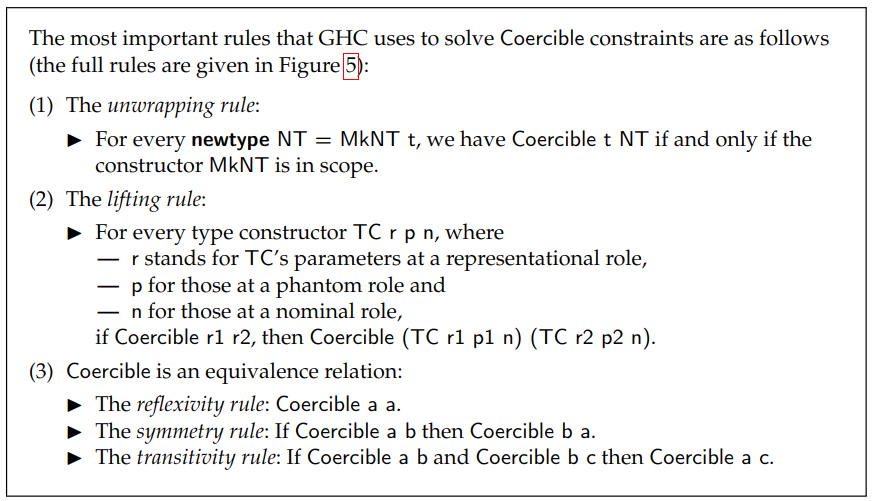
\includegraphics[width=\linewidth]{figs/coersions}
    \caption{Принципы построения инстансов \mintinline{haskell}|Coercible|~\cite{breitner2014safe}.}
    \label{fig:coersions}
\end{figure}

Теперь, можем избавиться от лишней трансформации списка:
\begin{minted}{haskell}
    linesH :: Html -> [Html]
    linesH = coerce lines
\end{minted}

Безопасность коерций обеспечивает \vocab{система ролей}.
Каждый типовой параметр имеет специальное свойство --- роль.

Роль phantom имеют фантомные типовые параметры.
Их можно свободно коерсить (нет пререквизитов для инстансов \mintinline{haskell}|Coercible|):
\begin{minted}{haskell}
    data Phantom h = Phantom
    data NestedPhantom b = MkNP [Phantom b] | SomethingElse

    instance Coercible (Phantom a) (Phantom b)
    instance Coercible (NestedPhantom a) (NestedPhantom b)
\end{minted}

Типовой параметр имеет роль representational, если типовой конструктор можно коерсить только при условии, что можно коерсить аргументы:
\begin{minted}{haskell}
    data Maybe a = Nothing | Just a
    instance Coerce a b => Coerce (Maybe a) (Maybe b)
\end{minted}

Роль nominal имеет типовой параметр, если типовой конструктор можно коерсить только при условии, что аргументы эквивалентны.
Это требуется, если типовой аргумент индексирует семейство или констреинт.
\begin{minted}{haskell}
    type family F a
    data Applied a = Applied (F a)
    instance (a ?$\sim$? b) => Coercible (Applied a) (Applied b)

    data ShowDict a where
      ShowDict :: Show a => a -> ShowDict a
    instance (a ?$\sim$? b) => Coercible (ShowDict a) (ShowDict b)
\end{minted}

Иногда компилятор выводит неправильную роль типовому параметру.
Например, если инварианты структуры зависят на конкретную имплементацию какого-то класса типов для типового аргумента, что совершенно не видно в декларации самого типа.
В таком случае, роли можно указать явно:
\begin{minted}{haskell}
    type role Map nominal representational
    data Map k v = ...
\end{minted}

Подробнее можно прочитать в~\cite{breitner2014safe} и~\cite[глава 8]{maguire-types}.

\subsubsection{Type reflection}

Рефлексия --- это языковой механизм получения информации о типах во время исполнения (на уровне термов).
Звучит знакомо, и действительно Haskell реализует этот механизм с интерфейсом классов типов~\cite{peyton2016reflection}.

Библиотека предоставляет магический класс типов \href{https://hackage.haskell.org/package/base-4.20.0.1/docs/Type-Reflection.html}{\mintinline{haskell}|Typeable|}, который реализуется компилятором для каждого конкретного типа.
Чтобы получить информацию о типе, в скоупе должен быть инстанс \mintinline{haskell}|Typeable| для этого типа.
Структура типа представлена типом-суммы \href{https://hackage.haskell.org/package/ghc-internal-9.1001.0/docs/src/GHC.Internal.Data.Typeable.Internal.html#TypeRep}{\mintinline{haskell}|TypeRep|}, который предоставляет возможность дополнительного типового контроля с помощью обобщённых алгебраических типов данных и типовых тегов.
\begin{minted}{haskell}
    class Typeable a where
      typeRep :: TypeRep a
\end{minted}

Например, следующим образом можно получить имя конструктора типа:
\begin{minted}{haskell}
    typeName :: forall a. Typeable a => String
    typeName = tyConName $ typeRepTyCon $ typeRep $ Proxy @a

    ghci> typeName @Int
\end{minted}

\begin{task}
    Объявите класс типов, который позволяет распечатать список типов.
\end{task}

С помощью структуры представления типа и экзистенциальных типов в Haskell можно эмулировать динамическую типизацию.
А именно: любой тип может быть преобразован в \href{}{\mintinline{haskell}|Dynamic|}, а потом безопасно преобразован обратно.
\begin{minted}{haskell}
    data Dynamic where
      Dynamic :: Typeable a => a -> Dynamic

    fromDynamic :: Typeable a => Dynamic -> Maybe a
\end{minted}

Это может быть полезно для определения гетерогенного хранилища ключ-значение:
\begin{minted}{haskell}
    data Store = Map Key Dynamic
    data Ref ty = Ref Key
    get :: Store -> Ref ty -> ty
\end{minted}

\subsubsection{Data reflection}

Как мы обсуждали ранее, в свойство когерентности гарантирует, что каждому типу в Haskell соответствует ровно один инстанс определённого класса типов.
И единственный способ объявить инстанс в Haskell --- декларацией на верхнем уровне, то есть он не может зависеть ни от каких локальных данных.
Однако в Haskell есть библиотека \href{https://hackage.haskell.org/package/reflection-2.1.6/docs/Data-Reflection.html}{Data.Reflection}\footnote{\url{https://www.tweag.io/blog/2017-12-21-reflection-tutorial/}}, которая позволяет создавать локальные инстансы для свежих, чёрной магией\footnote{\url{https://www.schoolofhaskell.com/user/thoughtpolice/using-reflection}} сгенерированных типов.

Она пользуется идеей ``поднятия значений в типы'', обсуждённой нами ранее (см.~\ref{subsubsec:reify}), но в несколько более общем виде.
Вместо заведения классов типов вида \mintinline{haskell}|Known_|, вводится один класс типов, индексированный типом термов \texttt{terms}, которые спускаются из типов:
\begin{minted}{haskell}
    class Reifies ty terms | ty -> terms where
      reflect :: Proxy ty -> terms
\end{minted}

Также библиотека умеет сгенерировать свежий тип и инстанс \mintinline{haskell}|Reifies|, который по этому свежему типу возвращает данное значение типа \texttt{a}.
Поскольку он передаётся в функцию высшего ранга, свежий тип не может утечь из скоупа~\cite[7.2, ST trick]{maguire-types}:
\begin{minted}{haskell}
    reify :: a -> (forall fresh . Reifies fresh a => Proxy fresh -> res) -> res
\end{minted}

Чтобы воспользоваться нестандартным инстансом класса типов для некого типа \texttt{a}, нужно объявить новый тип (например, с помощью \mintinline{haskell}|newtype|), содержащий данный, и написать для него нужный инстанс (см, например, \href{https://hackage.haskell.org/package/base-4.20.0.1/docs/Data-Ord.html#t:Down}{Down}).
Мы не хотим объявлять по новой декларации для каждого случая, поэтому заведём обёртку, похожую на \href{https://hackage.haskell.org/package/tagged-0.8.8/docs/Data-Tagged.html}{Data.Tagged}, которая позволяет добавлять фантомный типовой тег к типу значения.
Варьируя тег, можно получить сколь угодно много типов, оборачивающих данный.
\begin{minted}{haskell}
    newtype Wrapped tag a = Wrapped { unwrap :: a }
\end{minted}

Объявим тип обёртки \mintinline{haskell}|Wrapped tag a| представителем нужного класса типов.
Код для реализации будем с помощью \texttt{reflect} получать по типу тега в виде честного словаря.
\begin{minted}{haskell}
    data ReifiedOrd a = ReifiedOrd { compare :: a -> a -> Ordering }

    instance Reflect tag (ReifiedOrd a) => Ord (Wrapped tag a) where
      compare = coerce $ compare $ reflect $ Proxy @tag
\end{minted}

Наконец, можем вызвать функцию сортировки, подменив локально порядок на обратный:
\begin{minted}{haskell}
    sort :: Ord a => [a] -> [a]

    sortReverse :: forall a . Ord a => [a] -> [a]
    sortReverse xs =
      let dict = ReifiedOrd { compare = flip compare } in
      reify dict \(Proxy :: Proxy fresh) ->
        coerce $ sort @(Wrapped fresh a) $ coerce xs
\end{minted}

\subsubsection{Открытые структуры}

В динамических языках можно создавать объекты на ходу, последовательно дописывая в них содержимое, и не вводя предварительно декларацию.
В Haskell тоже так можно, используя пары для произведений и \mintinline{haskell}|Either| для сумм.
Однако у такой реализации есть два недостатка.
Первый --- эффективность, о более эффективных реализациях можно почитать в~\cite[глава 11]{maguire-types}.

Другой недостаток --- не очень гибкая типизация.
А именно --- порядок полей имеет значение и на типах в Haskell нет отношения подтипизации (например, нельзя передать значение с меньшим количеством полей или вариантов).
Но можно заметить, что констреинты лишены этих недостатков.
Поэтому можно организовывать тип структуры данных, например, таким образом:
\begin{minted}{haskell}
    (Int, Double) ?$\rightsquigarrow$? (Member Int d, Member Double d) => Prod d
\end{minted}

Далее мы вернёмся снова к открытым суммам, потому что они являются важной частью типизации расширяемых интерпретаторов~\cite{swierstra2008data}.

\subsubsection{Легковесные частичные стек-трейсы}

Забавной эксплуатацией классов типов в Haskell являются легковесные частичные стек-трейсы\footnote{\url{https://downloads.haskell.org/ghc/latest/docs/users_guide/exts/callstack.html}}.
Вообще для сбора трейсов нужна поддержка рантайма, что в случае Haskell усложняется ещё и тем, что модель вычислений, редукция графов, реальных трейсов не содержит и их приходится эмулировать.
Для легковесных трейсов же не требуется поддержка рантайма.

В GHC определён класс типов \mintinline{haskell}|GHC.Stack.HasCallStack|, позволяющий получить информацию о месте вызова функции.
Эту информацию фактически размещает компилятор в процессе вывода инстансов.
Если в месте вызова доступна информация с уровня выше, компилятор распространяет её дальше.
Таким образом, доступна информация только на определённую глубину стека вызовов.
\begin{minted}{haskell}
    myHead :: HasCallStack => [a] -> a
    myHead []     = error "empty"
    myHead (x:xs) = x

    bad :: Int
    bad = myHead []

    ghci> bad
    *** Exception: empty
    CallStack (from HasCallStack):
      error, called at Bad.hs:8:15 in main:Bad
      myHead, called at Bad.hs:12:7 in main:Bad
      -- no information about bad here
\end{minted}
